%%%%%%%%%%%%%%%%%%%%%%%%%%%%%%%%%%%%%%%%%
% a0poster Portrait Poster
% Efficient Attention for TinyCLIP: GQA / MQA K/V sharing
% University of Twente
%%%%%%%%%%%%%%%%%%%%%%%%%%%%%%%%%%%%%%%%%

\documentclass[a0,portrait]{a0poster}

\usepackage{multicol}
\columnsep=36pt
\columnseprule=3pt
\usepackage[svgnames]{xcolor}
\usepackage{times}
\usepackage{graphicx}
\graphicspath{{figures/}}
\usepackage{booktabs}
\usepackage{multirow}
\usepackage[font={small,color=NavyBlue},labelfont={bf,color=NavyBlue}]{caption}
\renewcommand{\normalsize}{\fontsize{28}{34}\selectfont}
\usepackage{amsfonts, amsmath, amsthm, amssymb}
\usepackage{wrapfig}
\usepackage[most]{tcolorbox}
\usepackage{colortbl}
\usepackage[table]{xcolor}

\makeatletter
\renewcommand\section{\@startsection{section}{1}{\z@}%
  {-0.7ex \@plus -0.4ex \@minus -.2ex}{0.3ex \@plus .2ex}{\normalfont\large\bfseries}}
\renewcommand\subsection{\@startsection{subsection}{2}{\z@}%
  {-0.6ex \@plus -0.4ex \@minus -.2ex}{0.2ex \@plus .2ex}{\normalfont\normalsize\bfseries}}
\makeatother

\setlength{\abovecaptionskip}{4pt}
\setlength{\belowcaptionskip}{0pt}
\setlength{\tabcolsep}{5pt}
\renewcommand{\arraystretch}{0.92}

\newcommand{\headerbox}[1]{%
\begin{tcolorbox}[colback=blue!10, arc=12pt, boxrule=0pt,
  left=6pt,right=6pt,top=6pt,bottom=6pt]
\large \textbf{#1}
\end{tcolorbox}}

\begin{document}

%----------------------------------------------------------------------------------------
%	POSTER HEADER
%----------------------------------------------------------------------------------------

\begin{minipage}[b]{\linewidth}
\centering
\VeryHuge \color{NavyBlue} \textbf{Efficient Attention for TinyCLIP} \\
\vspace{0.3cm}
\Huge \color{NavyBlue} \textbf{Grouped-Query and Multi-Query K/V Sharing} \\
\vspace{0.9cm}
\large \texttt{Rushat Gabhane} \quad \texttt{[teammates]} \\
\vspace{0.3cm}
\large University of Twente --- Foundation Models, Final Project
\end{minipage}

\vspace{0.5cm}

%----------------------------------------------------------------------------------------

\begin{multicols}{2}
\sloppy

%----------------------------------------------------------------------------------------
%	ABSTRACT
%----------------------------------------------------------------------------------------

\color{Black}
\section*{\Large{ABSTRACT}}
\vspace{-1cm}
\noindent\rule{\linewidth}{1pt}

We replace multi-head attention (MHA) in a pretrained \textbf{TinyCLIP-8M} with grouped-query (GQA) and multi-query (MQA) attention in \emph{both} the image and text encoders, by mean-pooling each group's key/value heads --- the conversion recipe of Ainslie et al.~\cite{gqa2023}. Raw conversion collapses zero-shot accuracy (56.8\% $\rightarrow$ $\sim$5\%), but a short feature-distillation \textbf{uptrain} recovers most of it: GQA-2 reaches \textbf{93\% of MHA accuracy on CIFAR-100 with half the K/V parameters}. Crucially, on a bidirectional \emph{encoder} the saving is parameter count only --- throughput and peak memory are unchanged, because there is no autoregressive KV-cache to shrink. A useful negative result: GQA's headline efficiency benefit does not transfer to CLIP-style encoders.

%----------------------------------------------------------------------------------------
%	INTRODUCTION
%----------------------------------------------------------------------------------------

\color{Black}
\section*{\Large INTRODUCTION \& PROBLEM STATEMENT}
\vspace{-1cm}
\noindent\rule{\linewidth}{1pt}

Multi-query~\cite{mqa2019} and grouped-query~\cite{gqa2023} attention reduce the number of key/value heads to speed up large-language-model \emph{decoding}, where the KV-cache dominates memory bandwidth. CLIP~\cite{clip2021} and its distilled variant TinyCLIP~\cite{tinyclip2023} are instead built from bidirectional \textbf{encoders}. \emph{Whether K/V sharing helps CLIP-style encoders is unexplored} --- the gap this work addresses.

\vspace{0.5cm}
\noindent\textbf{Main RQ:} Can MHA in TinyCLIP be replaced by GQA/MQA, and what is the accuracy--efficiency trade-off?
\vspace{0.4cm}
\begin{itemize}\setlength\itemsep{0pt}\setlength\topsep{0pt}\setlength\parsep{0pt}\setlength\partopsep{0pt}
    \item \textbf{SRQ1:} How much zero-shot accuracy is lost when K/V heads are pooled, and can a short uptrain recover it?
    \item \textbf{SRQ2:} Do parameter savings translate into runtime/memory savings on an encoder?
\end{itemize}

%----------------------------------------------------------------------------------------
%	METHOD
%----------------------------------------------------------------------------------------

\section*{\Large METHOD}
\vspace{-1cm}
\noindent\rule{\linewidth}{1pt}

\noindent\textbf{Model.} Pretrained \textbf{TinyCLIP-8M} (ViT, patch-16; 4 attention heads per encoder, head dim 64), via OpenCLIP.

\vspace{0.4cm}
\noindent\textbf{Conversion.} For each block, partition the 4 K/V heads into $G$ groups and \textbf{mean-pool} within each group; queries and the output projection are copied unchanged. $G=4$ is MHA (lossless), $G=2$ is GQA-2, $G=1$ is MQA. Applied to \emph{both} encoders.

\vspace{0.4cm}
\noindent\textbf{Uptrain.} Brief fine-tuning of the converted model by distilling image \emph{and} text features from the original MHA model (cosine loss, 1000 steps, CIFAR-10$+$CIFAR-100 images and class prompts).

\vspace{0.4cm}
\noindent\textbf{Evaluation.} Zero-shot top-1 on CIFAR-10/100; image-encoder throughput, peak GPU memory, and K/V parameter count (single GPU, fp16).

%----------------------------------------------------------------------------------------
%	RESULTS
%----------------------------------------------------------------------------------------

\section*{\Large RESULTS}
\vspace{-1cm}
\noindent\rule{\linewidth}{3pt}

\headerbox{Zero-shot accuracy: conversion collapses, uptraining recovers}
\vspace{0.4cm}

\begin{center}
\begin{tabular}{lccccc}
\toprule
\textbf{Method} & \textbf{K/V heads} & \textbf{Converted} & \textbf{Uptrained} & \textbf{CIFAR-10} & \textbf{CIFAR-100} \\
\midrule
MHA   & 4 & 56.8 & \textbf{56.8} & 72.3 & 41.3 \\
GQA-2 & 2 & 5.9  & \textbf{43.5} & 48.7 & 38.4 \\
MQA   & 1 & 5.0  & \textbf{28.7} & 31.7 & 25.6 \\
\bottomrule
\end{tabular}
\captionof{table}{\small\color{NavyBlue} Average zero-shot top-1 (\%). Conversion alone is near-random; uptraining restores GQA-2 to 77\% of MHA overall and \textbf{93\% on CIFAR-100}.}
\end{center}

\begin{center}\vspace{0.15cm}
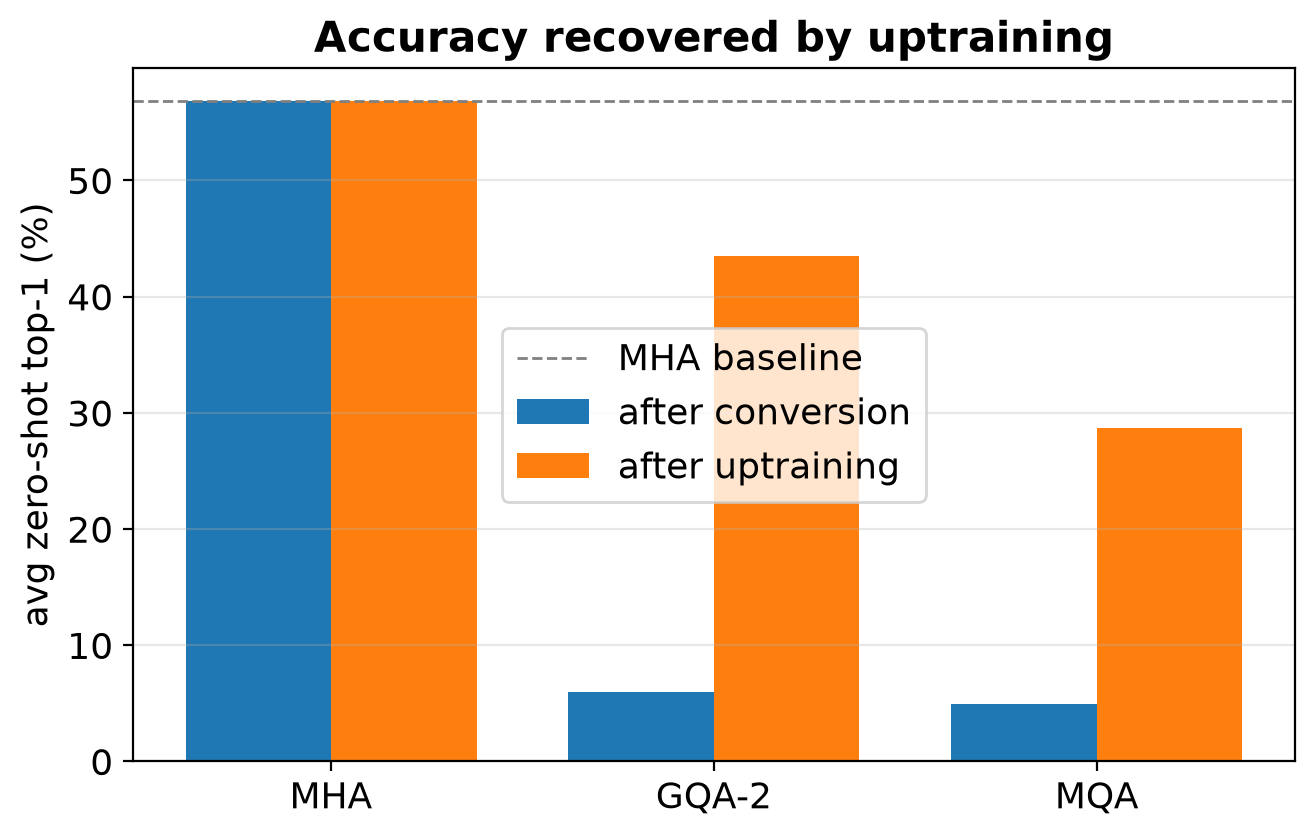
\includegraphics[width=\linewidth]{accuracy_recovery_tinyclip-8m.png}
\captionof{figure}{\small\color{NavyBlue} Average zero-shot top-1 after conversion vs.\ after uptraining. Dashed line: MHA baseline. A short uptrain closes most of the gap for GQA-2.}
\vspace{0.15cm}
\end{center}

\headerbox{Efficiency: K/V parameters shrink, runtime does not}
\vspace{0.4cm}

\begin{center}
\begin{tabular}{lccccc}
\toprule
\textbf{Method} & \textbf{K/V params} & \textbf{Total} & \textbf{Throughput} & \textbf{Peak mem} & \textbf{p50} \\
 & & \textbf{params} & \textbf{(img/s)} & \textbf{(MB)} & \textbf{(ms)} \\
\midrule
MHA   & 1.71M (100\%) & 23.4M & 6069 & 337 & 10.47 \\
GQA-2 & 0.86M (\textbf{50\%}) & 22.6M & 6089 & 336 & 10.46 \\
MQA   & 0.43M (\textbf{25\%}) & 22.2M & 6250 & 335 & 10.17 \\
\bottomrule
\end{tabular}
\captionof{table}{\small\color{NavyBlue} K/V projection parameters drop 2$\times$/4$\times$, but total params, throughput and peak memory are essentially flat.}
\end{center}

\begin{center}\vspace{0.15cm}
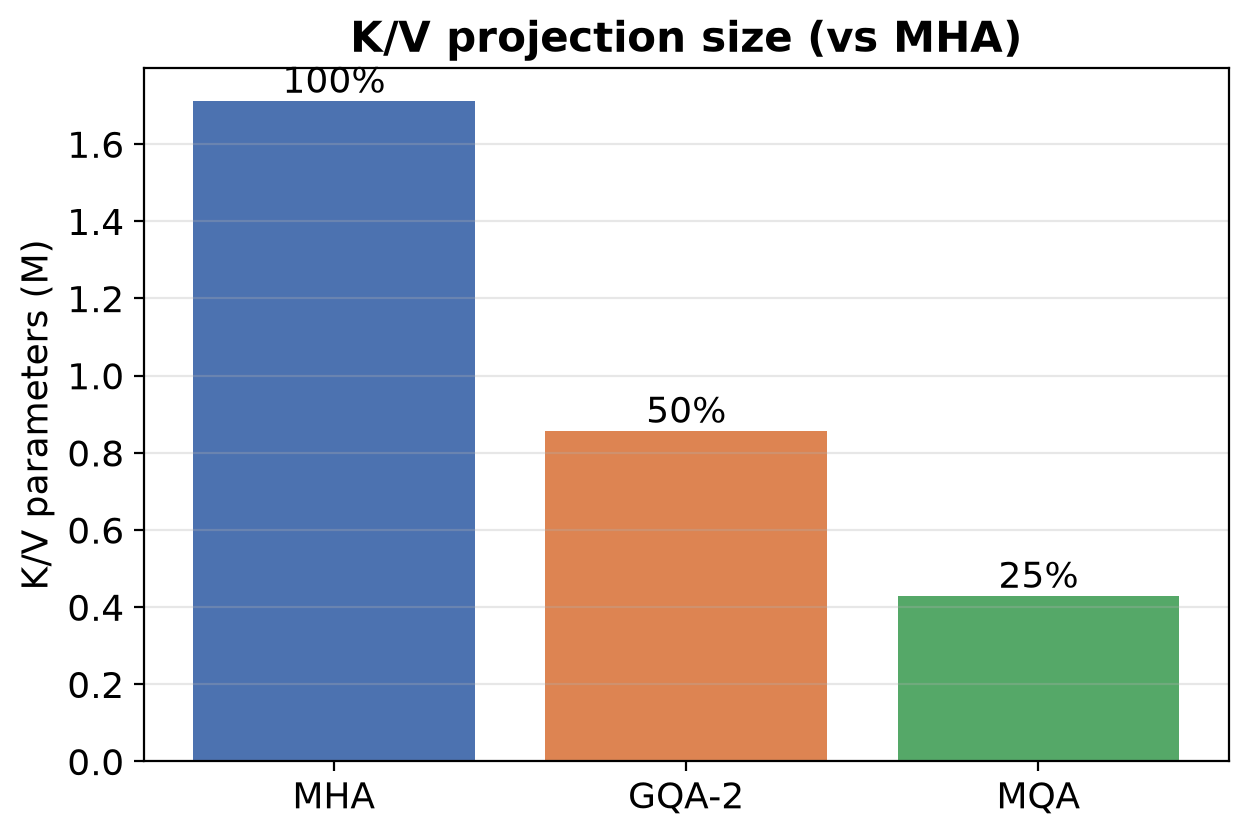
\includegraphics[width=\linewidth]{kv_compression_tinyclip-8m.png}
\captionof{figure}{\small\color{NavyBlue} K/V projection size relative to MHA: 100\% / 50\% / 25\%.}
\vspace{0.15cm}
\end{center}

\begin{center}\vspace{0.15cm}
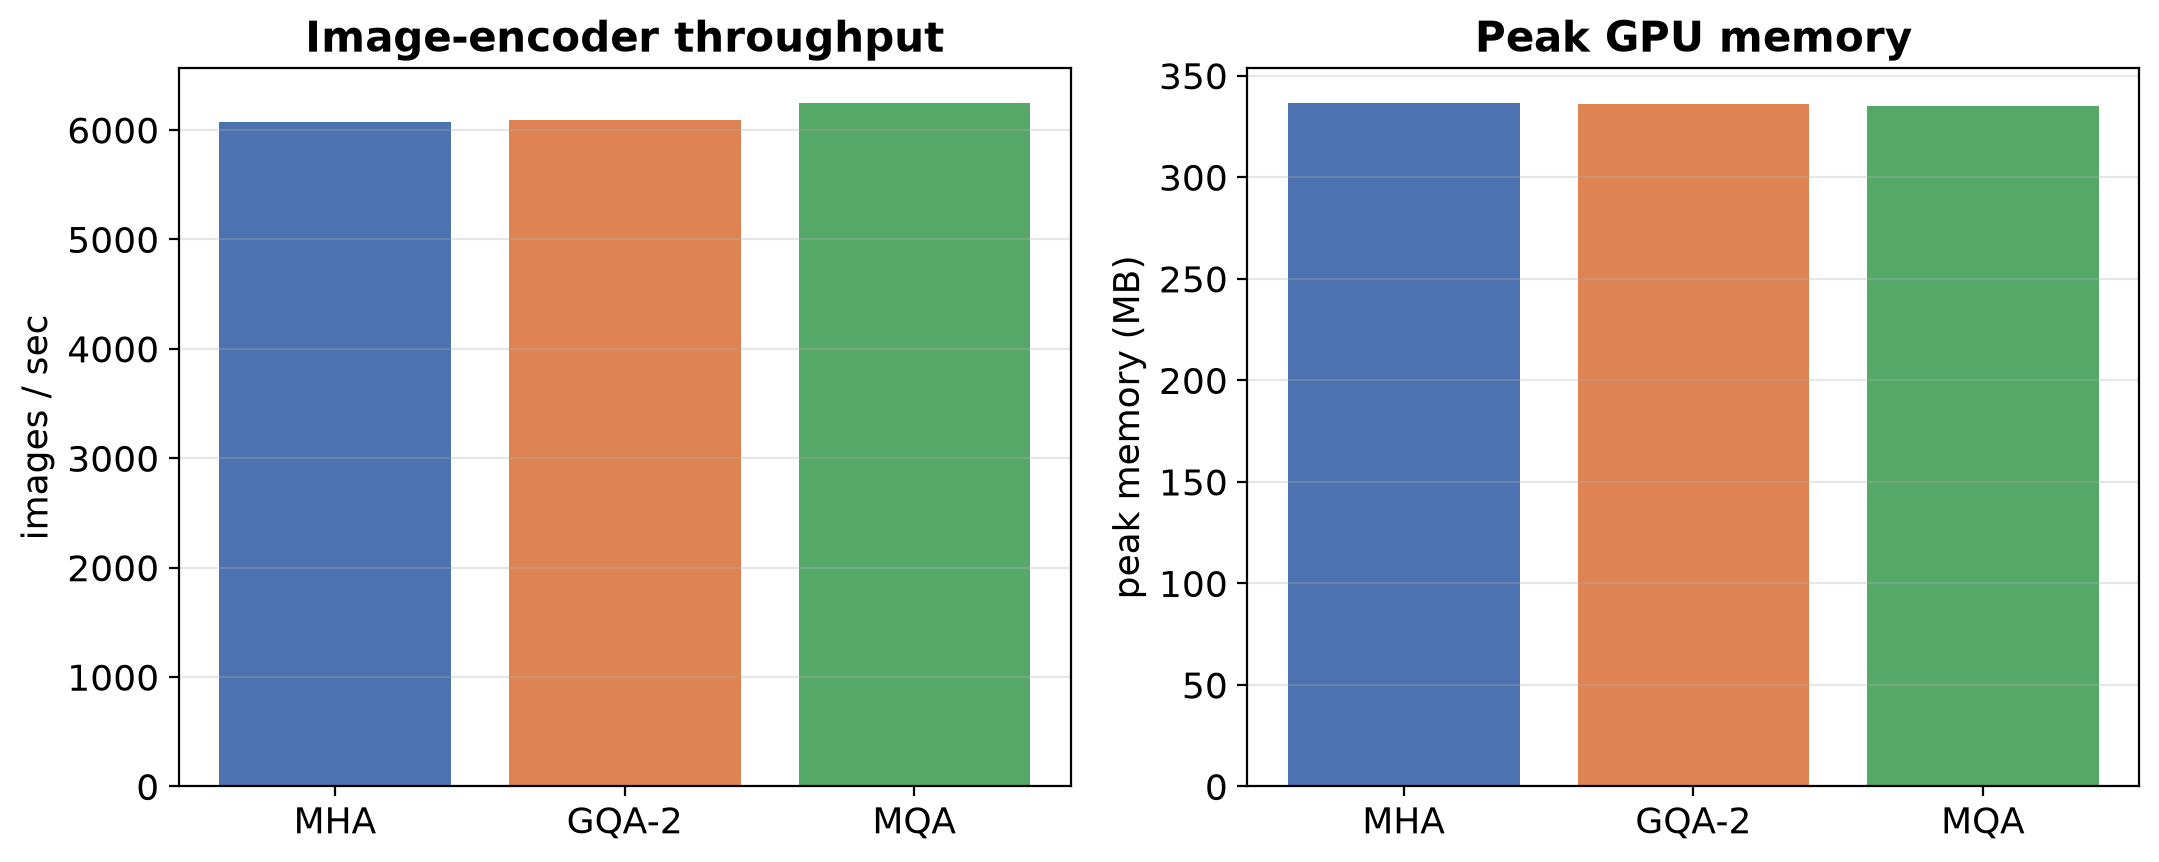
\includegraphics[width=\linewidth]{throughput_memory_tinyclip-8m.png}
\captionof{figure}{\small\color{NavyBlue} Image-encoder throughput and peak GPU memory are nearly identical across variants --- the parameter saving does not become a runtime saving.}
\vspace{0.15cm}
\end{center}

\begin{center}\vspace{0.15cm}
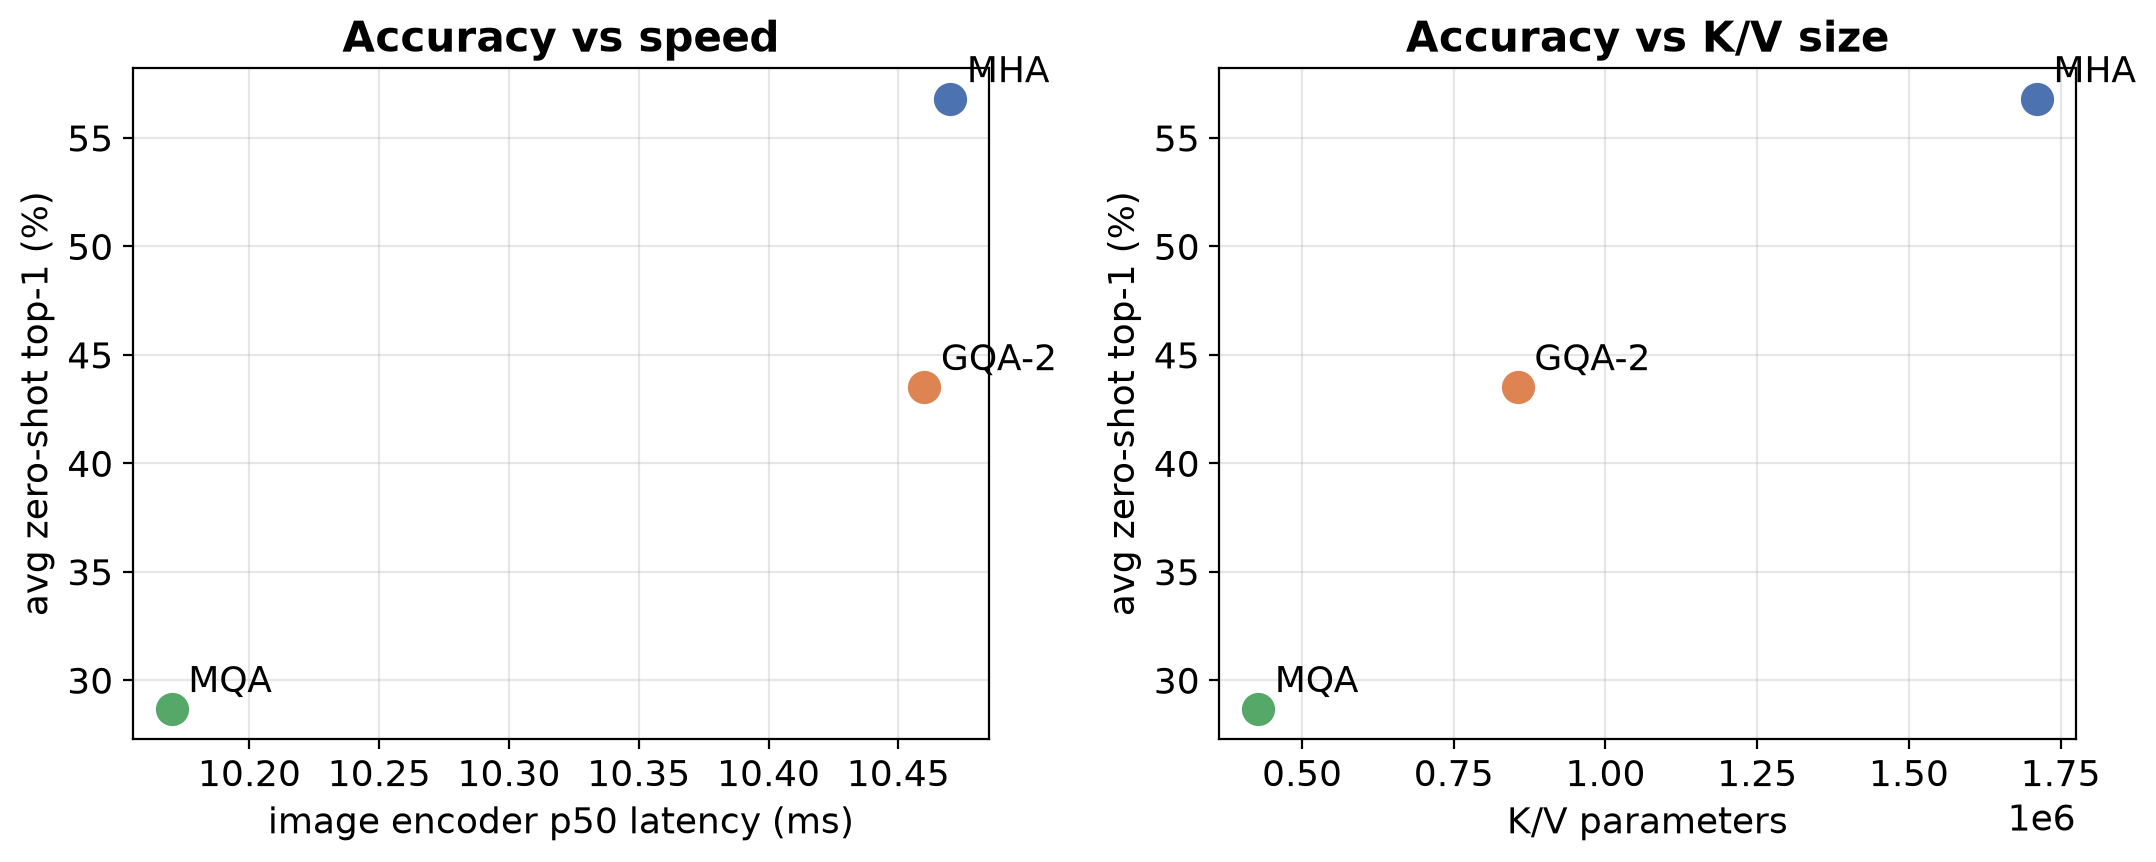
\includegraphics[width=\linewidth]{tradeoff_tinyclip-8m.png}
\captionof{figure}{\small\color{NavyBlue} Accuracy vs.\ cost. GQA-2 is the favorable point (half the K/V params, $\sim$77\% accuracy); MQA is too aggressive for a 4-head model.}
\vspace{0.15cm}
\end{center}

\headerbox{Why no runtime win? Encoder vs.\ decoder}
GQA/MQA save memory by shrinking the \textbf{KV-cache during autoregressive decoding}. A CLIP encoder is \textbf{bidirectional and runs in a single pass --- it has no KV-cache}. The GQA paper itself applies GQA only to the decoder, never the encoder~\cite{gqa2023}. On CLIP, the only real saving is the K/V projection weights (a small slice of the model), and broadcasting K/V back to full width leaves attention FLOPs unchanged.

%----------------------------------------------------------------------------------------
%	CONCLUSIONS
%----------------------------------------------------------------------------------------

\color{Black}
\section*{\Large CONCLUSIONS}
\vspace{-1cm}
\noindent\rule{\linewidth}{1pt}

\begin{itemize}\setlength\itemsep{0pt}\setlength\topsep{0pt}\setlength\parsep{0pt}\setlength\partopsep{0pt}
    \item \textbf{Conversion alone collapses} zero-shot accuracy on a small CLIP; \textbf{a short uptrain recovers most of it}.
    \item \textbf{GQA-2 is the sweet spot}: $\sim$77\% of MHA overall and \textbf{93\% on CIFAR-100 at half the K/V parameters}; MQA trades far more accuracy for 4$\times$ compression.
    \item On a bidirectional encoder the benefit is \textbf{parameter compression only} --- no throughput or memory gain, because there is no KV-cache.
    \item \textbf{Takeaway / negative result:} GQA/MQA's efficiency motivation does not transfer to CLIP encoders; it is a model-size lever, not a speed lever.
    \item \textbf{Future work:} larger TinyCLIP (more heads $\rightarrow$ finer GQA sweep), longer uptraining, and vision-only vs.\ both-encoder ablation.
\end{itemize}
\color{Black}

%----------------------------------------------------------------------------------------
%	REFERENCES
%----------------------------------------------------------------------------------------

{\tiny\raggedright\setlength{\parskip}{1pt}
\begin{thebibliography}{9}
\bibitem{gqa2023} Ainslie et al., ``GQA: Training Generalized Multi-Query Transformer Models from Multi-Head Checkpoints,'' \textit{EMNLP}, 2023.
\bibitem{mqa2019} Shazeer, ``Fast Transformer Decoding: One Write-Head is All You Need,'' arXiv:1911.02150, 2019.
\bibitem{clip2021} Radford et al., ``Learning Transferable Visual Models From Natural Language Supervision,'' \textit{ICML}, 2021.
\bibitem{tinyclip2023} Wu et al., ``TinyCLIP: CLIP Distillation via Affinity Mimicking and Weight Inheritance,'' \textit{ICCV}, 2023.
\end{thebibliography}
}

\end{multicols}
\end{document}
